%%%%%%%%%%%%%%%%%%%%%%%%%%%%%%%%%%%%%%%%%
% Beamer Presentation
% LaTeX Template
% Version 1.0 (10/11/12)
%
% This template has been downloaded from:
% http://www.LaTeXTemplates.com
%
% License:
% CC BY-NC-SA 3.0 (http://creativecommons.org/licenses/by-nc-sa/3.0/)
%
%%%%%%%%%%%%%%%%%%%%%%%%%%%%%%%%%%%%%%%%%
	
%----------------------------------------------------------------------------------------
%	PACKAGES AND THEMES
%----------------------------------------------------------------------------------------

\documentclass{beamer}

\mode<presentation> {

% The Beamer class comes with a number of default slide themes
% which change the colors and layouts of slides. Below this is a list
% of all the themes, uncomment each in turn to see what they look like.

%\usetheme{default}
%\usetheme{AnnArbor}
%\usetheme{Antibes}
%\usetheme{Bergen}
%\usetheme{Berkeley}
\usetheme{Berlin}
%\usetheme{Boadilla}
%\usetheme{CambridgeUS}
%\usetheme{Copenhagen}
%\usetheme{Darmstadt}
%\usetheme{Dresden}
%\usetheme{Frankfurt}
%\usetheme{Goettingen}
%\usetheme{Hannover}
%\usetheme{Ilmenau}
%\usetheme{JuanLesPins}
%\usetheme{Luebeck}
%\usetheme{Madrid}
%\usetheme{Malmoe}
%\usetheme{Marburg}
%\usetheme{Montpellier}
%\usetheme{PaloAlto}
%\usetheme{Pittsburgh}
%\usetheme{Rochester}
%\usetheme{Singapore}
%\usetheme{Szeged}
%\usetheme{Warsaw}

% As well as themes, the Beamer class has a number of color themes
% for any slide theme. Uncomment each of these in turn to see how it
% changes the colors of your current slide theme.

%\usecolortheme{albatross}
\usecolortheme{beaver}
%\usecolortheme{beetle}
%\usecolortheme{crane}
%\usecolortheme{dolphin}
%\usecolortheme{dove}
%\usecolortheme{fly}
%\usecolortheme{lily}
%\usecolortheme{orchid}
%\usecolortheme{rose}
%\usecolortheme{seagull}
%\usecolortheme{seahorse}
%\usecolortheme{whale}
%\usecolortheme{wolverine}

%\setbeamertemplate{footline} % To remove the footer line in all slides uncomment this line
%\setbeamertemplate{footline}[page number] % To replace the footer line in all slides with a simple slide count uncomment this line

%\setbeamertemplate{navigation symbols}{} % To remove the navigation symbols from the bottom of all slides uncomment this line
}

\usepackage{graphicx} % Allows including images
\usepackage{booktabs} % Allows the use of \toprule, \midrule and \bottomrule in tables
\usepackage{graphicx, subcaption}
\usepackage{amssymb, mathtools}
\usepackage{algorithm, algpseudocode}
\usepackage{amsmath}
\usepackage[absolute,overlay]{textpos}

%
\captionsetup{labelformat=empty,labelsep=none}

%
\DeclarePairedDelimiter{\inner}{\langle}{\rangle}

% 
\usepackage{adjustbox}
\usepackage{tikz}
\usetikzlibrary{positioning,shapes.geometric, arrows, fit,calc}
\tikzstyle{block} = [draw, rectangle, fill=orange!50, text width=8em, text centered, minimum height=15mm, node distance=10em]
\tikzstyle{container} = [draw, rectangle, dashed, inner sep=0.7em]
\tikzstyle{arrow} = [thick,->,>=stealth]

%macros from Bob Gray
\usepackage{"./macro/GrandMacros"}
\usepackage{"./macro/Macro_BIO235"}

\usepackage[normalem]{ulem}

\addtobeamertemplate{navigation symbols}{}{%
    \usebeamerfont{footline}%
    \usebeamercolor[fg]{footline}%
    \hspace{1.2em}%
    \insertframenumber/\inserttotalframenumber
}
\setbeamercolor{footline}{fg=gray}
\makeatletter
\let\@@magyar@captionfix\relax
\makeatother
%----------------------------------------------------------------------------------------
%	TITLE PAGE
%----------------------------------------------------------------------------------------

\AtBeginSection[]{%
\begin{frame}
    \tableofcontents[currentsection]
\end{frame}
}

\begin{document}

\title{Robust Bootstrap Testing for Nonlinear Effect  \\ 
with Kernel Ensemble}
\author{\textbf{Wenying Deng}\\ 
Department of Biostatistics \\
Harvard University}
\date{Biostat Seminar \\ October 18, 2018}
\begin{frame}
\titlepage
\begin{tiny}
*joint work with Jeremiah Liu and Brent Coull, with help and suggestions from Dr. Erin Lake.
\end{tiny}
\end{frame}

\begin{frame}
\frametitle{Contents} % Table of contents slide, comment this block out to remove it
\tableofcontents[hideallsubsections]
% Throughout your presentation, if you choose to use \section{} and \subsection{} commands, these will automatically be printed on this slide as an overview of your presentation
\end{frame}

%----------------------------------------------------------------------------------------
%	PRESENTATION SLIDES
%----------------------------------------------------------------------------------------
\section{Problem Setup} 

\begin{frame}
\frametitle{Problem Setup}
\begin{itemize}[<+->]
\item Data: 
$$\{ y_i, \bx_i \}_{i=1}^n, \quad \mbox{where} \quad 
\bx_i= \{\bx_{i1}, \bx_{i2}\}$$
\begin{itemize}
\item Effect of $\bx_1$ and $\bx_2$ are nonlinear.
\end{itemize}
\item Model:
$$y_i=\mu + f_1(\bx_{i1})+ f_2(\bx_{i2})+\epsilon_i$$
\item Question: Does $\bx_{2}$ have any impact on $y$? or
$$ H_0: \quad f_2(\bx_{i2}) = 0$$
\item Example: Consider a treatment effect study for lung cancer:
\begin{enumerate}
\item $y$: Lab measure for lung cancer
\item $\bx_1$: Nicotine intake
\item $\bx_2$: Treatment
\end{enumerate}
\end{itemize}
\end{frame}

\begin{frame}
\frametitle{How to do this?}
\begin{itemize}
\item Data: 
$$\{ y_i, \bx_i \}_{i=1}^n, \quad \mbox{where} \quad 
\bx_i= \{\bx_{i1}, \bx_{i2}\}$$
\begin{itemize}
\item Effect of $\bx_1$ and $\bx_2$ are nonlinear.
\end{itemize}
\item Model:
$$y_i=\mu + f_1(\bx_{i1})+ f_2(\bx_{i2})+\epsilon_i$$
\item Question: Does $\bx_{2}$ have any impact on $y$? or
$$ H_0: \quad f_2(\bx_{i2}) = 0$$
\item Example: Consider a treatment effect study for lung cancer:
\begin{enumerate}
\item $y$: Lab measure for lung cancer
\item $\bx_1$: Nicotine intake
\item $\bx_2$: Treatment
\end{enumerate}
\end{itemize}

\begin{textblock*}{0.5cm}(9.25cm,0.61\textheight)
${\color{red} \mathbf{\Rightarrow}}$
\end{textblock*}

\begin{textblock*}{3cm}(9.5cm,0.55\textheight)
\centering
{\color{red} Kernel Machine Regression}
\end{textblock*}
\end{frame}

\begin{frame}
\frametitle{How to do this?}
\begin{itemize}
\item Data: 
$$\{ y_i, \bx_i \}_{i=1}^n, \quad \mbox{where} \quad 
\bx_i= \{\bx_{i1}, \bx_{i2}\}$$
\begin{itemize}
\item Effect of $\bx_1$ and $\bx_2$ are nonlinear.
\end{itemize}
\item Model:
$$y_i=\mu + f_1(\bx_{i1})+ f_2(\bx_{i2})+\epsilon_i$$
\item Question: Does $\bx_{2}$ have any impact on $y$? or
$$ H_0: \quad f_2(\bx_{i2}) = 0$$
\item Example: Consider a treatment effect study for lung cancer:
\begin{enumerate}
\item $y$: Lab measure for lung cancer
\item $\bx_1$: Nicotine intake
\item $\bx_2$: Treatment
\end{enumerate}
\end{itemize}

\begin{textblock*}{0.5cm}(9.25cm,0.61\textheight)
${\color{red} \mathbf{\Rightarrow}}$
\end{textblock*}

\begin{textblock*}{3cm}(9.5cm,0.55\textheight)
\centering
{\color{red} Kernel Machine Regression}
\end{textblock*}

\begin{textblock*}{0.5cm}(10.85cm,0.66\textheight)
${\color{red} \mathbf{\Downarrow}}$
\end{textblock*}

\begin{textblock*}{3cm}(9.5cm,0.75\textheight)
\centering
{\color{red} Variance Component Test}
\end{textblock*}
\end{frame}

\section{Model $\&$ Method}
\subsection{Estimating $f$: Kernel Machine Regression (KMR)}
\begin{frame}
\frametitle{Kernel Machine Regression}
\begin{itemize}
\item Consider the typical linear model
$$y_i=\mu + x_i^\top \bbeta$$
\item In matrix notation:
$$\by = \bmu + \bX\bbeta$$
\end{itemize}
\vspace{2mm}

\begin{figure}
\centering
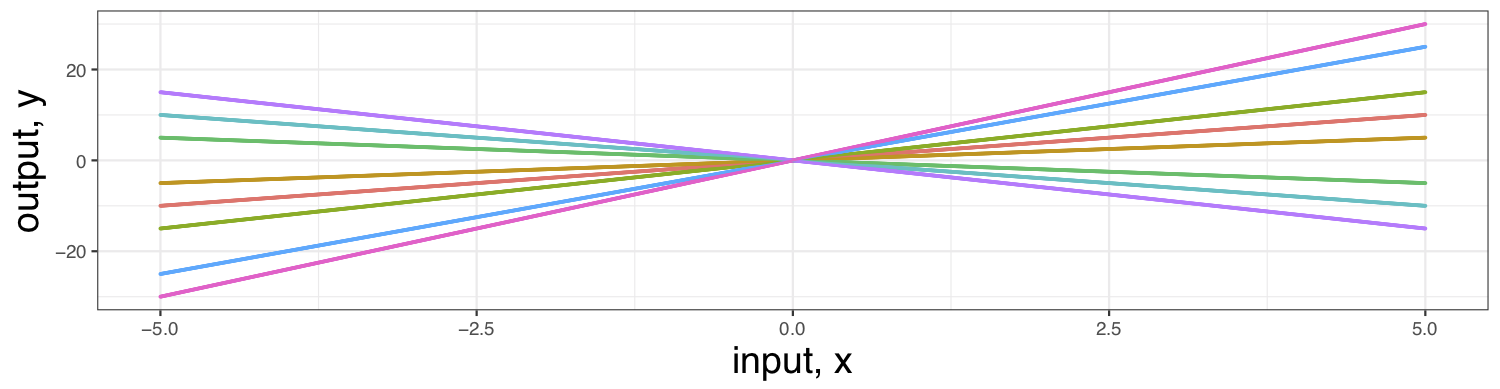
\includegraphics[width=.7\linewidth]{./plot/linear_axis} 
\caption{\textbf{Linear Model}: $y_i=\mu + x_i\beta$}
\end{figure}

\end{frame}

\begin{frame}
\frametitle{Kernel Machine Regression}
\begin{itemize}
\item A more general way to write this:
$$y_i=\mu + f(x_i) \qquad f(x_i)=\sum_{j=1}^n {\color{red} k(x_i, x_{j})}\alpha_{j}$$
\item In matrix notation:
$$\by = \bmu + \bK\balpha$$
\item Linear regression corresponds to $k(x_i, x_j)=(1+x_i^\top x_j)$.
\end{itemize}

\begin{figure}
\centering
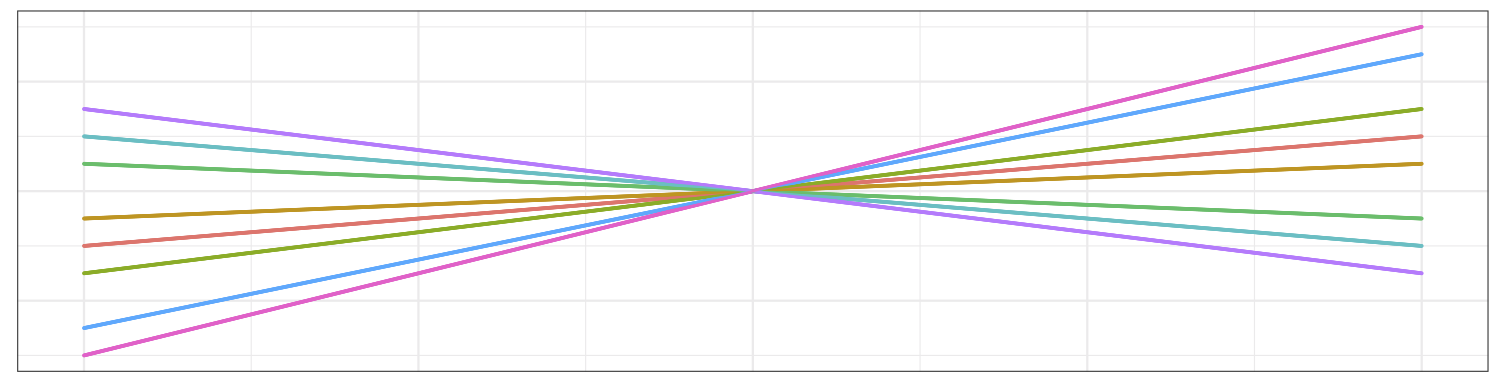
\includegraphics[width=.7\linewidth]{./plot/linear} 
\vspace{-0.2cm}
\caption{\textbf{Linear Kernel}: $k(x_i, x_j)=(1+x_i^\top x_j)$}
\end{figure}
\end{frame}

\begin{frame}
\frametitle{Example: Polynomial Kernels}
\begin{figure}
\centering
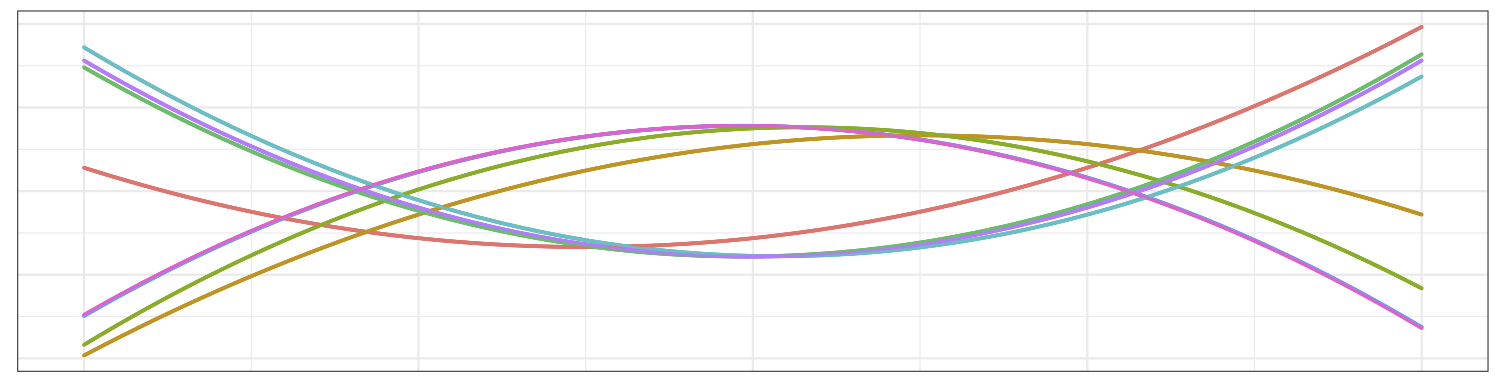
\includegraphics[width=.7\linewidth]{./plot/quad} 
\caption{\textbf{Quadratic Polynomial Kernel}: $k(x_i, x_j)=(1+x_i^\top x_j)^2$}
\end{figure}

\begin{figure}
\centering
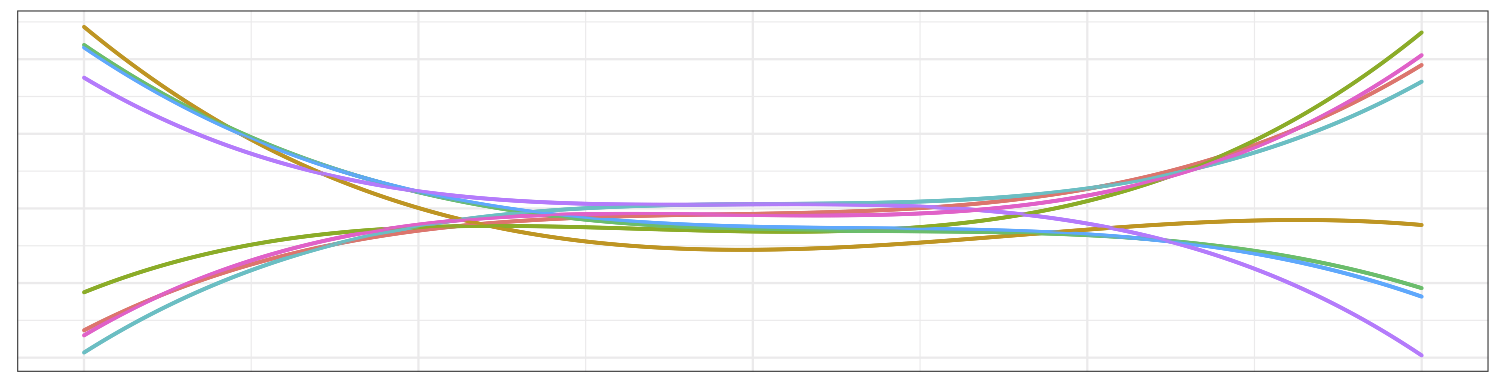
\includegraphics[width=.7\linewidth]{./plot/cubic} 
\caption{\textbf{Cubic Polynomial Kernel}: $k(x_i, x_j)=(1+x_i^\top x_j)^3$}
\end{figure}
\end{frame}

\begin{frame}
\frametitle{Example: (Really) Flexible Kernels}
\begin{figure}
\centering
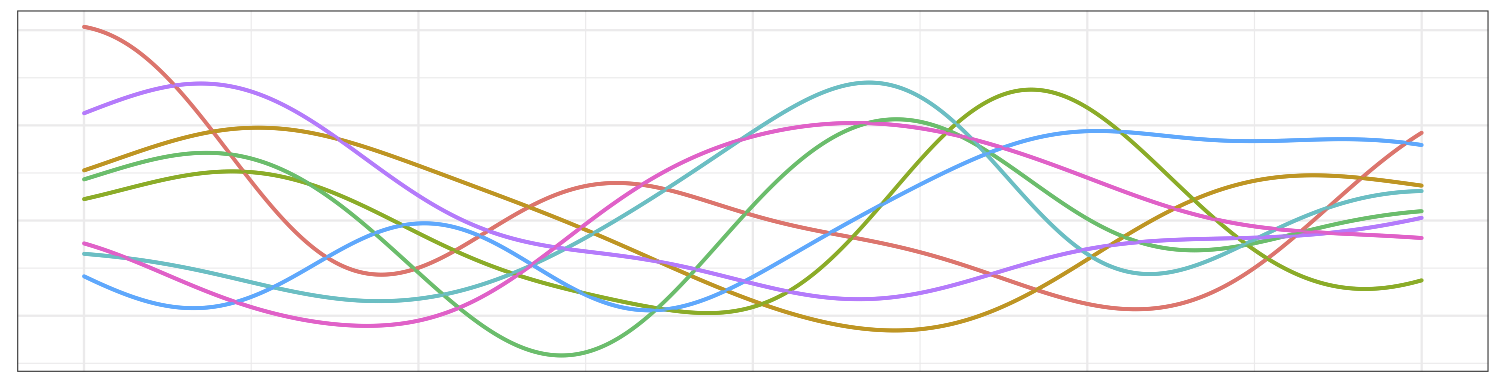
\includegraphics[width=.7\linewidth]{./plot/rbf2} 
\caption{\textbf{Radial Basis Functions}: $k(x_i, x_j)=\exp(-\frac{\lVert x_i - x_j \rVert^2}{2l^2})$}
\end{figure}

\begin{figure}
\centering
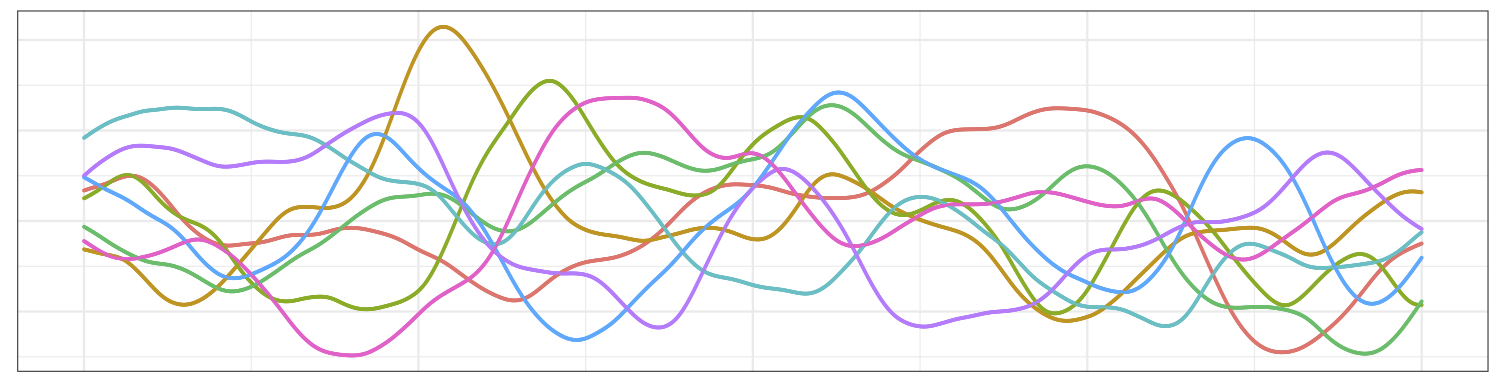
\includegraphics[width=.7\linewidth]{./plot/mat3_5} 
\caption{\textbf{Mat\'{e}rn 3/2 Kernel}: $(1+\frac{\sqrt{3} \lVert x_i - x_j \rVert}{l})\exp(-\frac{\sqrt{3} \lVert x_i - x_j \rVert}{l})$}
\end{figure}

\end{frame}

\subsection{Testing $f=0$: Variance Component Test}

\begin{frame}
\frametitle{KMR as a Linear Mixed Model}
As it turns out, KMR can be written as a Linear Mixed Model. \\
In the case of fitting $f(\bx)$:
\begin{itemize}
\item Kernel Machine Regression:
$$\by=\bmu + {\color{red}\bK} \balpha + \bepsilon$$
\item Linear Mixed Model:
\begin{align*}
\by &= \bmu + \bh + \bepsilon,\\
\bh &\sim \mathrm{N}(\mathbf{0}, {\color{red}\bK})
\end{align*}
\end{itemize}
\end{frame}

\begin{frame}
\frametitle{KMR as a Linear Mixed Model}
In the case of fitting $f_1(\bx_1) + f_2(\bx_2)$:
\begin{itemize}
\item Kernel Machine Regression:
$$\by=\bmu + {\color{red}(\bK_1 + \bK_2)}\balpha + \bepsilon$$
\item Linear Mixed Model:
\begin{align*}
\by &= \bmu + \bh + \bepsilon,\\
\bh &\sim \mathrm{N}(\mathbf{0}, {\color{red}\bK_1 + \bK_2})
\end{align*}
\end{itemize}
\end{frame}

\begin{frame}
\frametitle{Variance Component Test}
So if want to test for $H_0: f_2(\bx_2)=0$:
\begin{align*}
\by &= \bmu + \bh + \bepsilon,\\
\bh &\sim \mathrm{N}(\mathbf{0}, \bK_1 + {\color{red}\boldsymbol{\tau}}\bK_2)
\end{align*}

\begin{itemize}
\item Test Hypothesis: $$H_0: \boldsymbol{\tau}=0$$
\item Test Statistic: $$T \propto \hat{\bepsilon}^\top \bK_2 \hat{\bepsilon}$$
where $\hat{\bepsilon}=\by-\hat{\bmu} - \bK_1 \hat{\balpha}$ is null model residual.
\item Null Distribution: 
$$\hat{P}_0(T):= \mbox{distribution of}\; \; T \propto \hat{\bepsilon}^\top \bK_2 \hat{\bepsilon}\; \; \mbox{under the null}$$
\end{itemize}
\end{frame}


\begin{frame}
\frametitle{Summary}
\begin{itemize}
\item \textbf{Data}: 
$\{ y_i, \bx_i \}_{i=1}^n, \quad \mbox{where} \quad 
\bx_i= \{\bx_{i1}, \bx_{i2}\}$
\item \textbf{Goal}: Test for $$\quad H_0: \quad f_2(\bx_{i2}) = 0$$
\item \textbf{Model}: Kernel Machine Regression
$$\by =\bmu + \bK_1\balpha +\bepsilon$$
\item \textbf{Hypothesis Test}: Variance Component Test
$$ T \propto \hat{\bepsilon}^\top \bK_2 \hat{\bepsilon}$$
\item Looks like we solved everything! 
\begin{itemize}[<+->]
\item But this test doesn't always work in practice...
\item Why? Easy to misspecify null model $\by =\bmu + \bK_1\balpha$.
\item Hard to choose a proper kernel function $k$.
\item How to solve this? {\color{red} \textbf{Ensemble learning}!}
\end{itemize}
\end{itemize}
\end{frame}

\section{Cross-Validated Kernel Ensemble} 
\begin{frame}
\frametitle{The Kernel Misspecification Problem}
\begin{itemize}
\item If just use one kernel, hard to fit data correctly all the time.
\end{itemize}

\begin{figure}
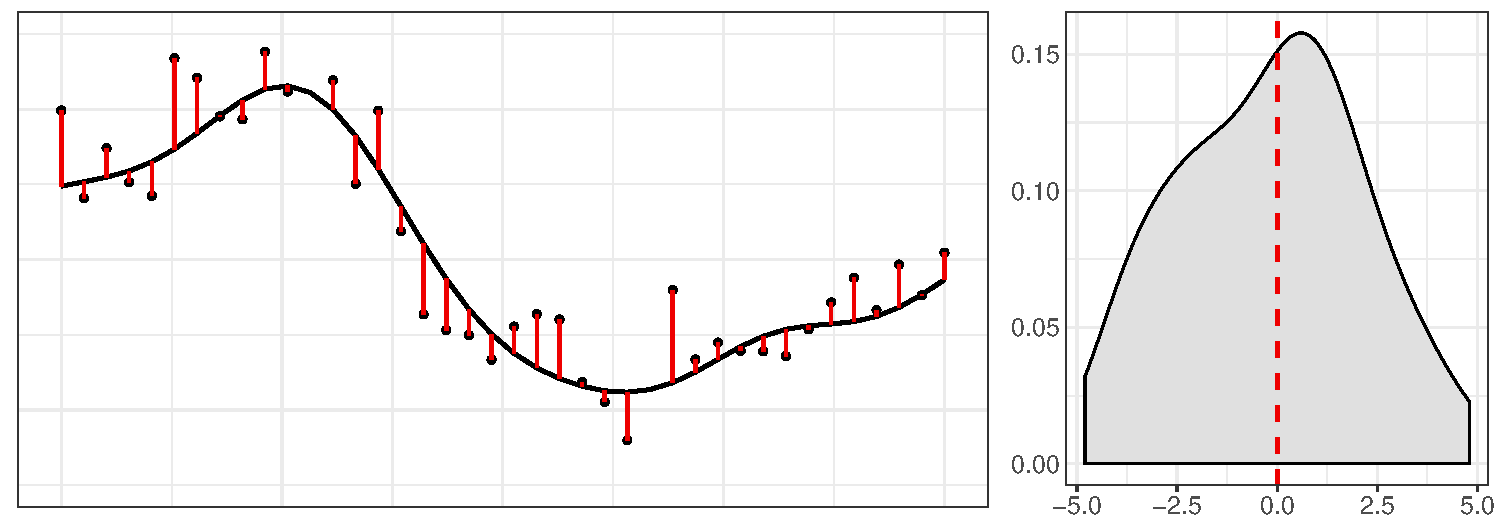
\includegraphics[height=3cm, width=10.5cm]{./plot/raw_final} 
\caption{Ideal model fit}
\end{figure}

\end{frame}

\begin{frame}
\frametitle{Motivation}
\begin{itemize}
\item Kernel too simple $\Rightarrow$ underfitting $\Rightarrow$ biased  residual estimate $\hat{\bepsilon}$.
\end{itemize}

\begin{figure}
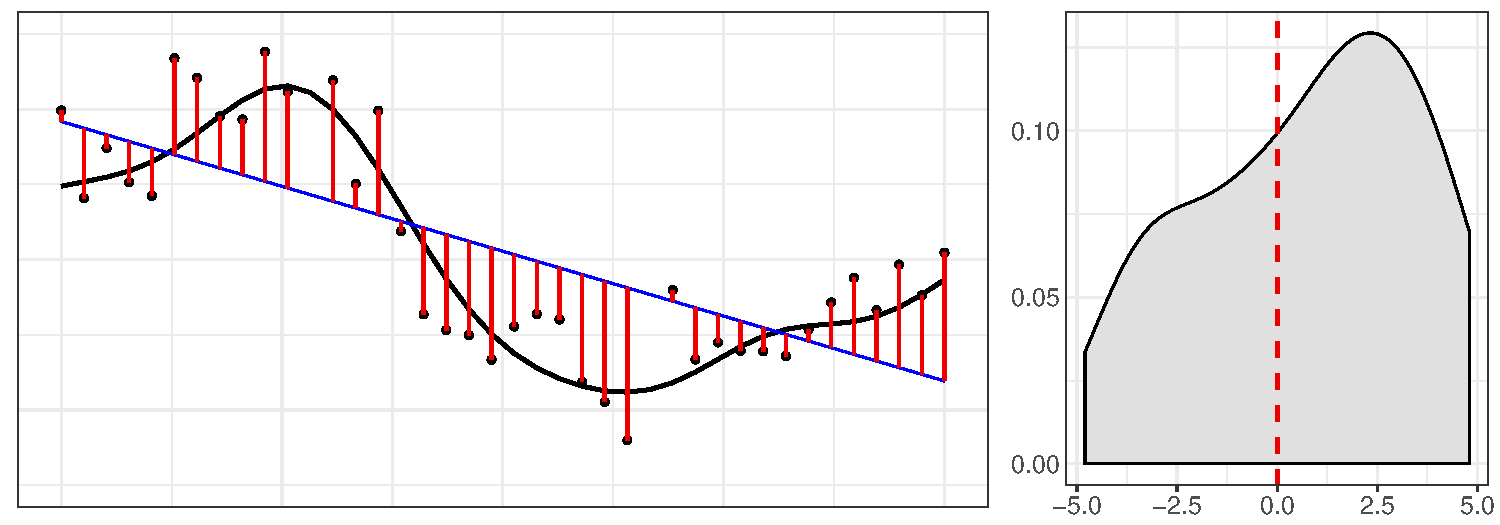
\includegraphics[height=3cm, width=10.5cm]{./plot/under_final} 
\caption{Underfit, biased $\hat{\bepsilon}$}
\end{figure}

\end{frame}

\begin{frame}
\frametitle{Motivation}
\begin{itemize}
\item Kernel too flexible $\Rightarrow$ overfitting $\Rightarrow$ under-estimated residual $\hat{\bepsilon}$.
\end{itemize}

\begin{figure}
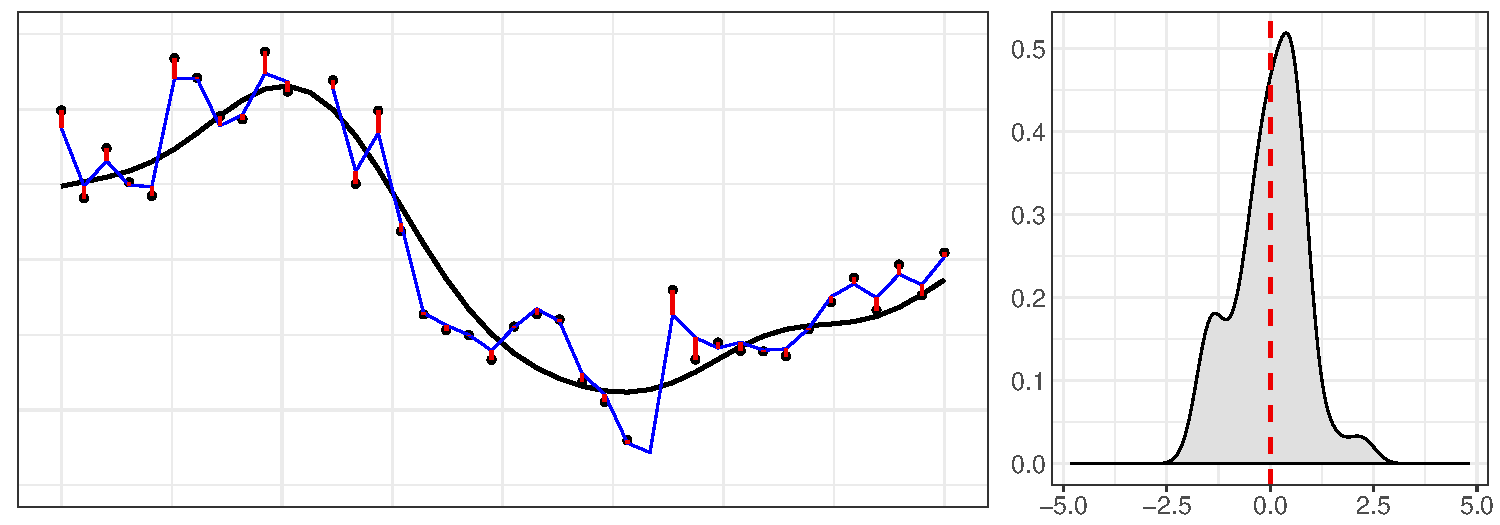
\includegraphics[height=3cm, width=10.5cm]{./plot/over_final} 
\caption{Overfit, under-estimated $\hat{\bepsilon}$}
\end{figure}

\end{frame}

\begin{frame}
\frametitle{Motivation}
\begin{itemize}
\item Incorrect $\hat{\bepsilon}$ $\Rightarrow$ incorrect $T \propto \hat{\bepsilon}^T\bK_2\hat{\bepsilon}$
$\Rightarrow$ incorrect inference!
\end{itemize}

\begin{itemize}
    \item[] 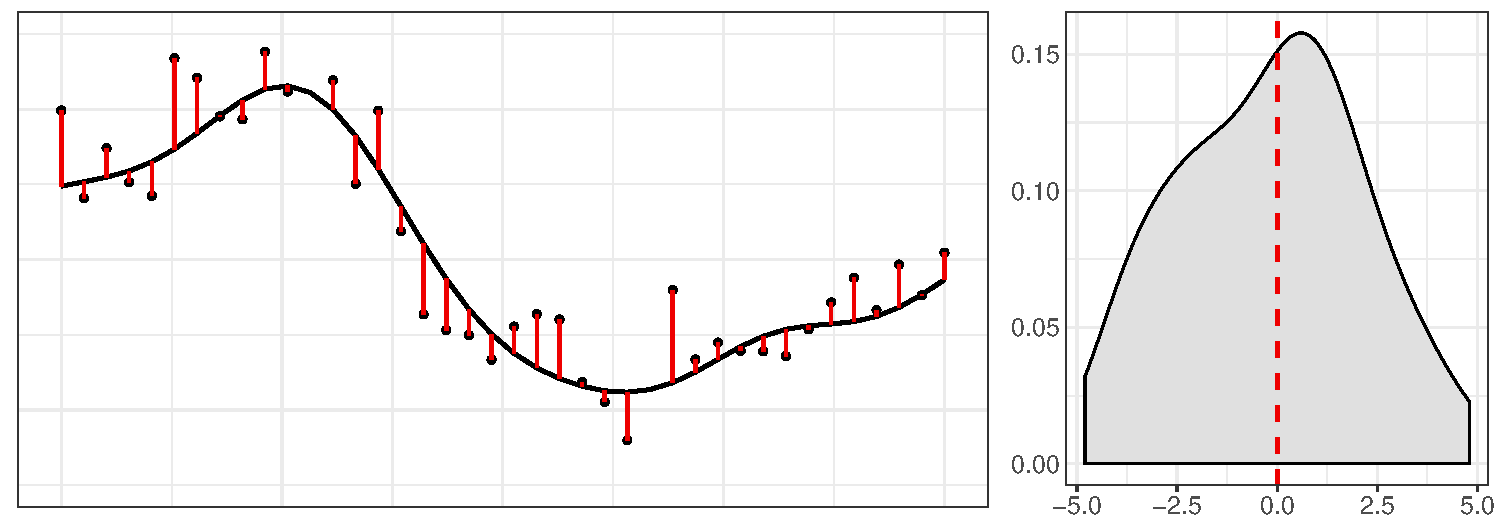
\includegraphics[height=1.8cm, width=10.5cm]{./plot/raw_final} 
    \item[] 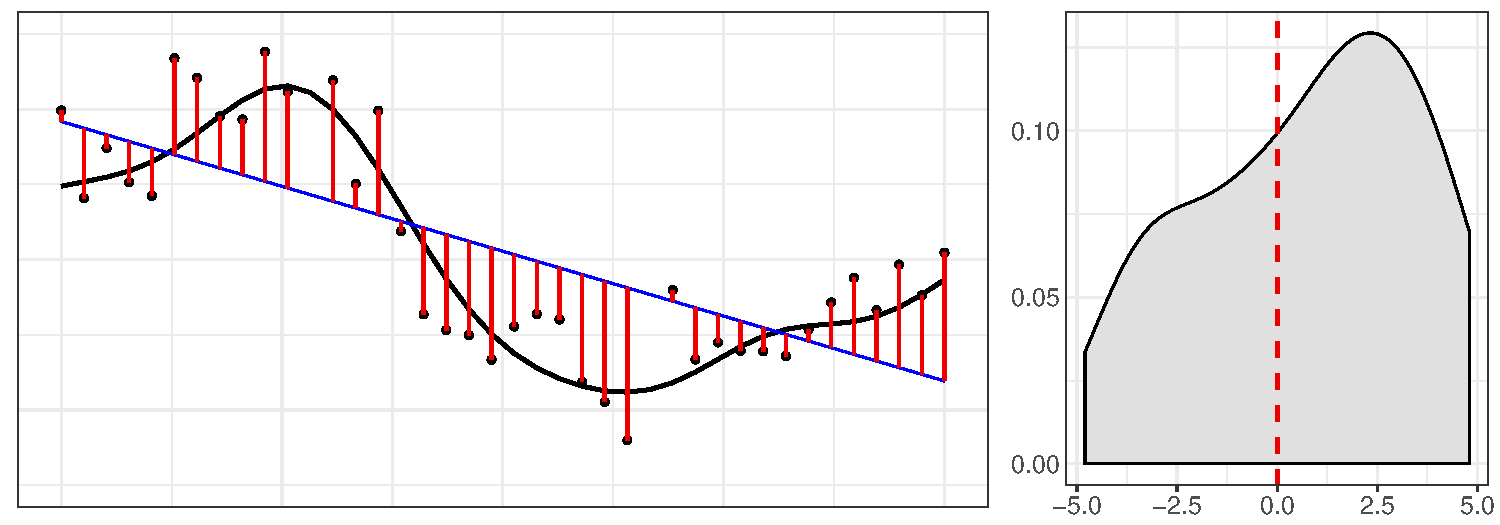
\includegraphics[height=1.8cm, width=10.5cm]{./plot/under_final} 
    \item[] 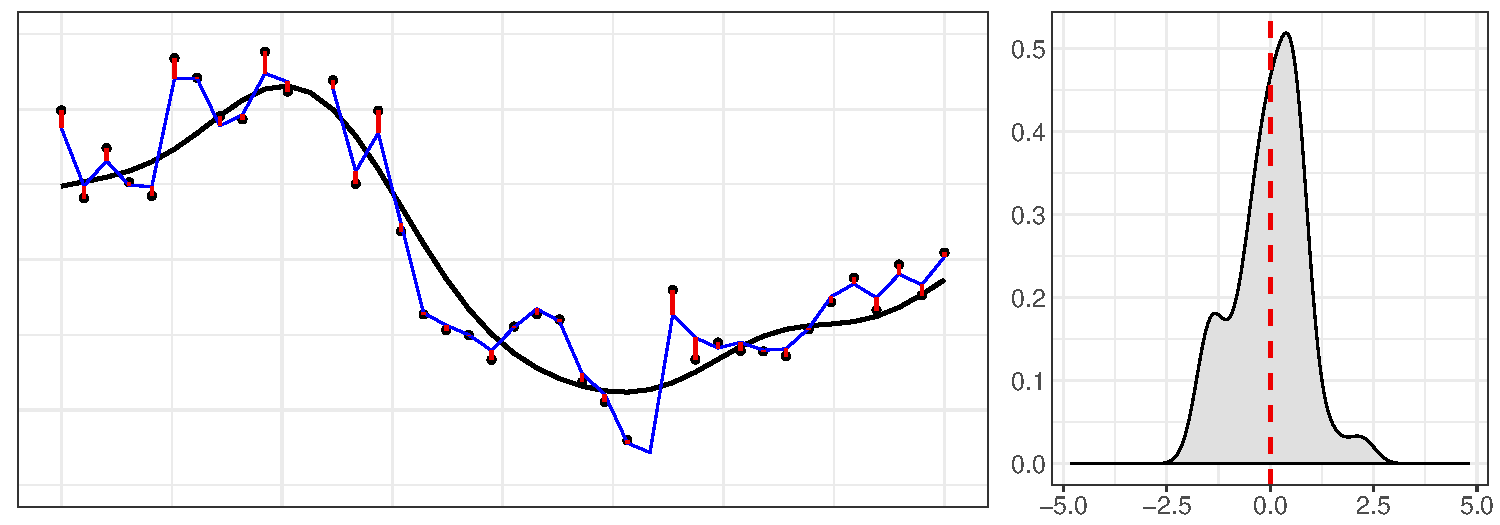
\includegraphics[height=1.8cm, width=10.5cm]{./plot/over_final} 
  \end{itemize}
\end{frame}

\begin{frame}
\frametitle{CVEK: Better $\hat{\epsilon}$ using Ensemble Learning}
\begin{itemize}
\item Idea: Try many possible kernels.
\end{itemize}
\vspace{1em}

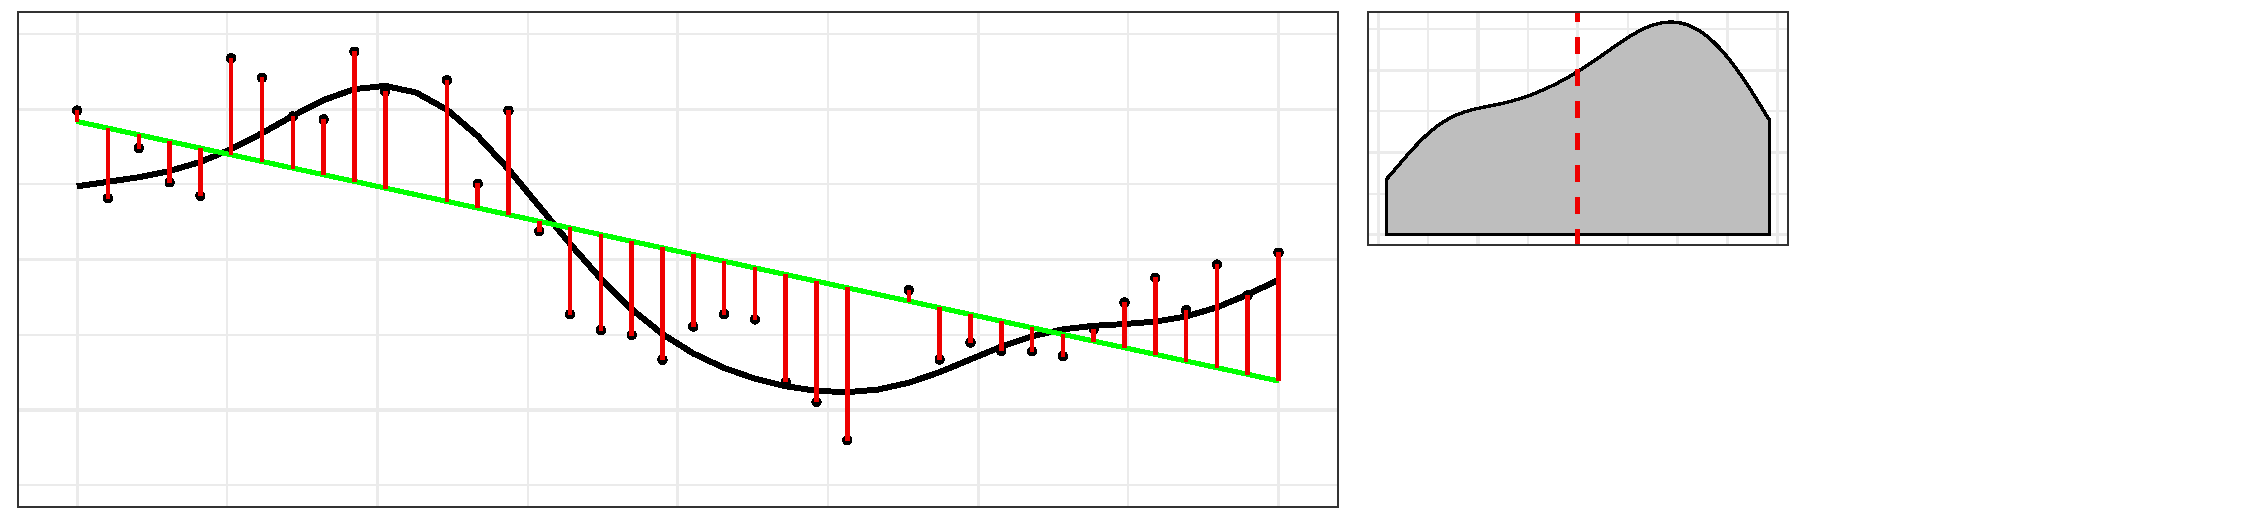
\includegraphics[width=\linewidth]{./plot/k1} 
\end{frame}

\begin{frame}
\frametitle{CVEK: Better $\hat{\epsilon}$ using Ensemble Learning}
\begin{itemize}
\item Idea: Try many possible kernels.
\end{itemize}
\vspace{1em}

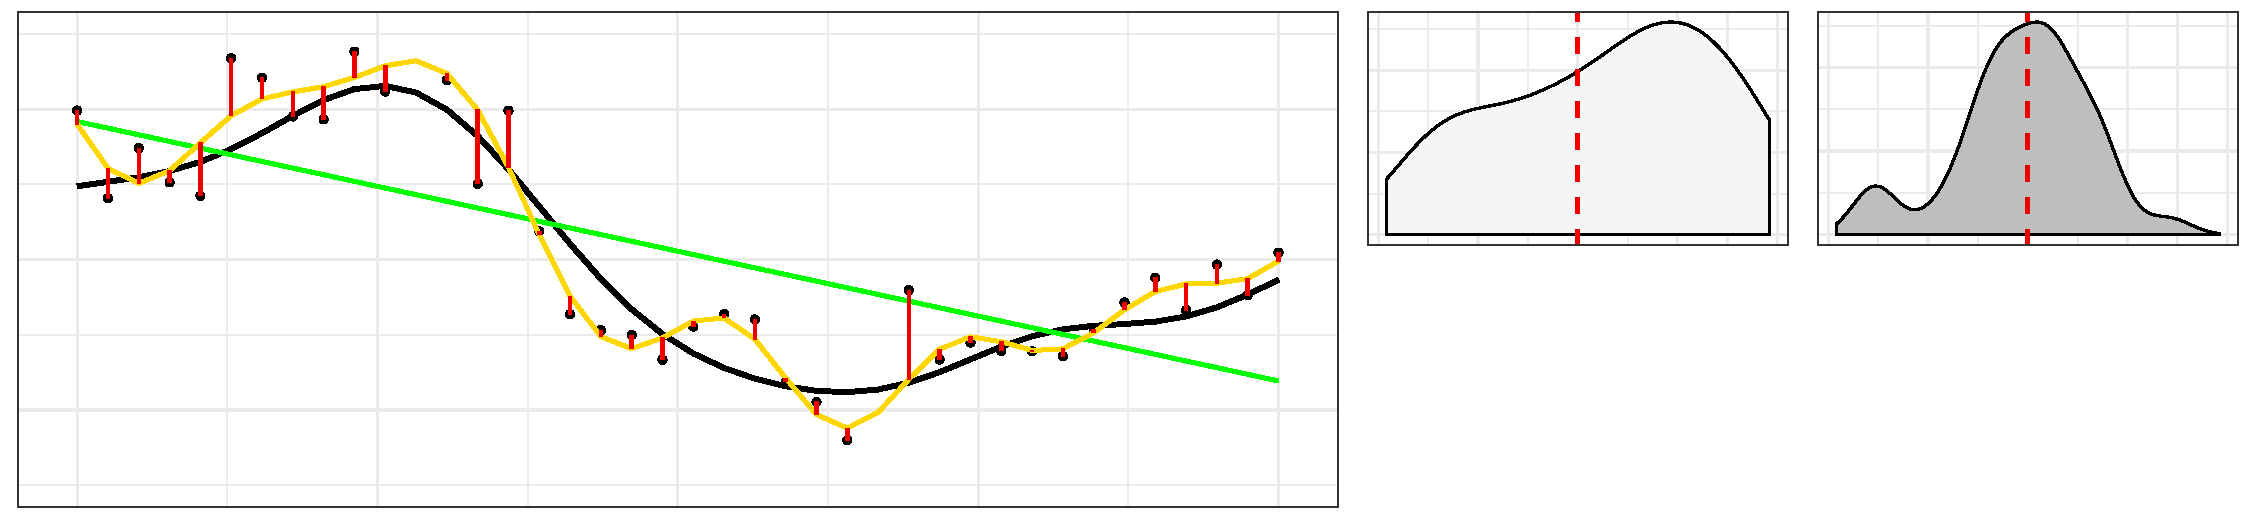
\includegraphics[width=\linewidth]{./plot/k2} 
\end{frame}

\begin{frame}
\frametitle{CVEK: Better $\hat{\epsilon}$ using Ensemble Learning}
\begin{itemize}
\item Idea: Try many possible kernels.
\end{itemize}
\vspace{1em}

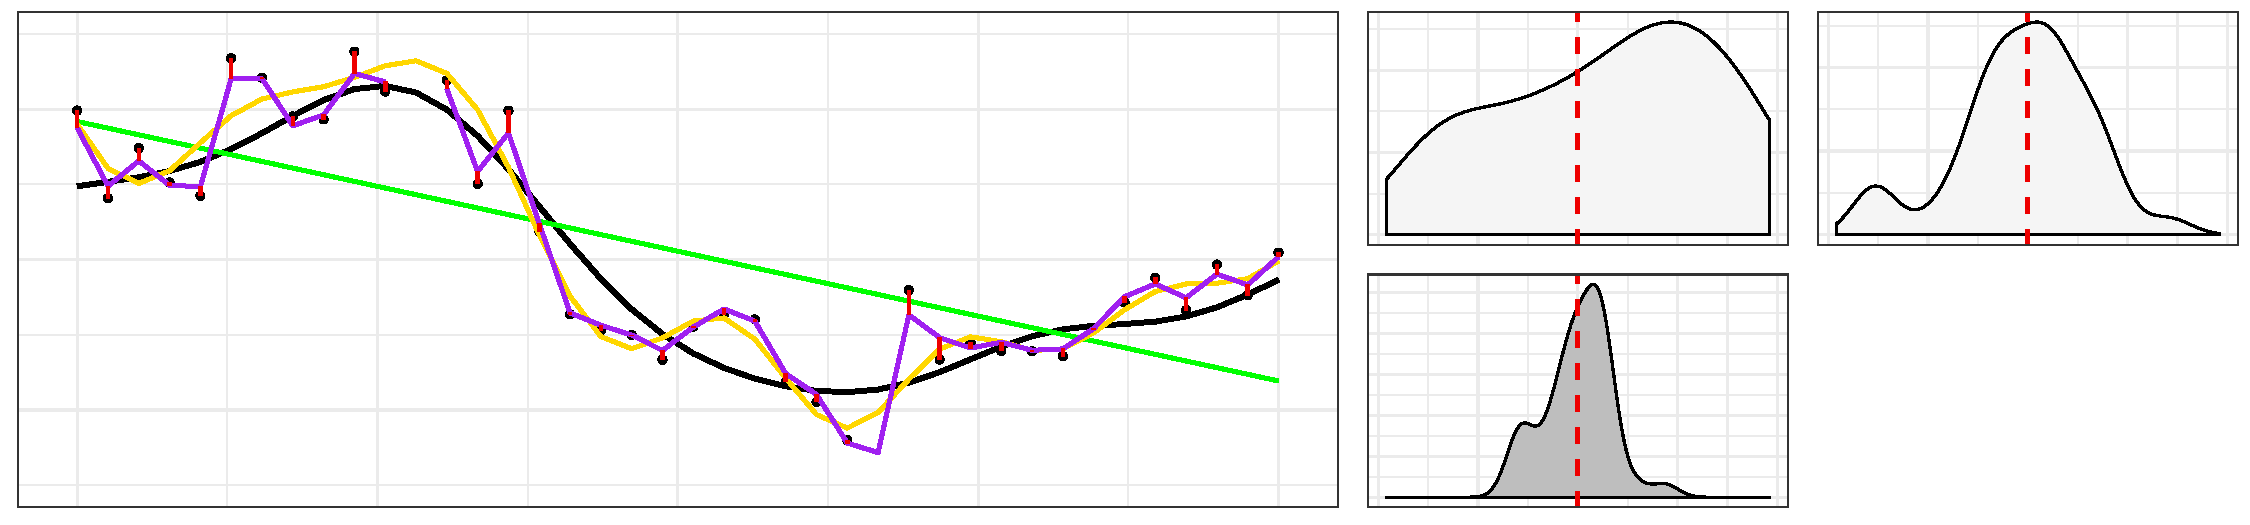
\includegraphics[width=\linewidth]{./plot/k3} 
\end{frame}

\begin{frame}
\frametitle{CVEK: Better $\hat{\epsilon}$ using Ensemble Learning}
\begin{itemize}
\item Combine them to produce proper model fit.
\begin{itemize}
\item based on individual kernel's \textbf{CV} performance.
\end{itemize}
\item Hence the name:
$$\mbox{\textbf{C}ross-\textbf{V}alidated \textbf{E}nsemble of \textbf{K}ernels}$$
\vspace{-.7cm}
\item Better model fit $\Rightarrow$ better residual estimate 
$\Rightarrow$ better inference!
\end{itemize}
\vspace{1em}
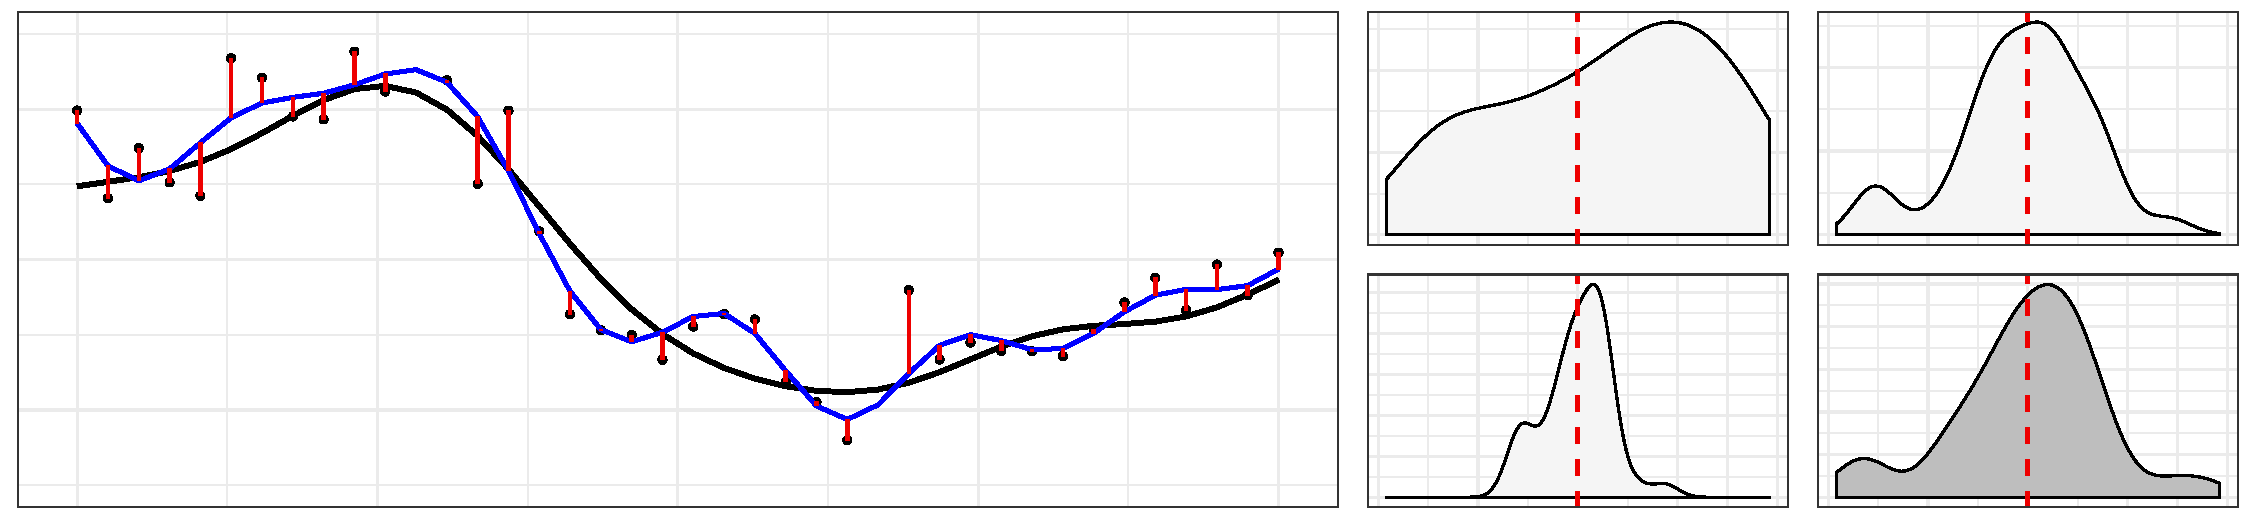
\includegraphics[width=0.9\linewidth]{./plot/k4} 
\end{frame}

\begin{frame}
\frametitle{Summary}
\begin{itemize}
\item \textbf{Data}: 
$\{ y_i, \bx_i \}_{i=1}^n, \quad \mbox{where} \quad 
\bx_i= \{\bx_{i1}, \bx_{i2}\}$
\item \textbf{Goal}: Test for $$\quad H_0: \quad f_2(\bx_{i2}) = 0$$
\item \textbf{Model}: {\color{red}\textbf{CVEK}}: Kernel Machine Regression + Ensemble Learning
$$\by =\bmu + \bK_1\balpha +\bepsilon$$
\item \textbf{Hypothesis Test}: Variance Component Test
$$ T \propto \hat{\bepsilon}^\top \bK_2 \hat{\bepsilon}$$
\item Looks like we solved everything! 
\begin{itemize}[<+->]
\item But still doesn't work super well in small sample...
\item Why? Asymptotic test replies on large-sample approximation.
\item How to solve this? {\color{red} \textbf{Bootstrap Test}!}
\end{itemize}
\end{itemize}
\end{frame}

\section{Bootstrap Test} 
\begin{frame}
\frametitle{Asymptotic v.s. Bootstrap Test}
\[\hat{P}_0(T):= \mbox{distribution of}\; \; \hat{\bepsilon}^\top \bK_2 \hat{\bepsilon}\; \;  \mbox{under the null:}\; \hat{\bepsilon}=\by-\hat{\bmu} - \bK_1 \hat{\balpha}\]
\begin{itemize}
\item Asymptotic
\begin{enumerate}
\item pretend $\hat{\bepsilon}$ come from $n \to \infty$ data
\item null distribution of $\hat{\bepsilon}$: $\hat{P}_{asym}(\hat{\bepsilon})$ is derived analytically
\item null distribution of $T$: $\hat{P}_{0}(\hat{\bepsilon}^\top \bK_2 \hat{\bepsilon})$
\end{enumerate}
\item Bootstrap
\begin{enumerate}
\item don't assume distribution of $\hat{\bepsilon}$, sample directly from empirical distribution
\item null distribution of $\hat{\bepsilon}$: $\hat{P}_{empirical}(\hat{\bepsilon})$ is estimated from bootstrap sample
\item null distribution of $T$: $\hat{P}_{0}(\hat{\bepsilon}^\top \bK_2 \hat{\bepsilon})$
\end{enumerate}
\end{itemize}
\end{frame}

\begin{frame}
\frametitle{Bootstrap Test: Idea}
\begin{enumerate}
    \item<+-> Given training sample 
    \begin{figure}
	\centering
    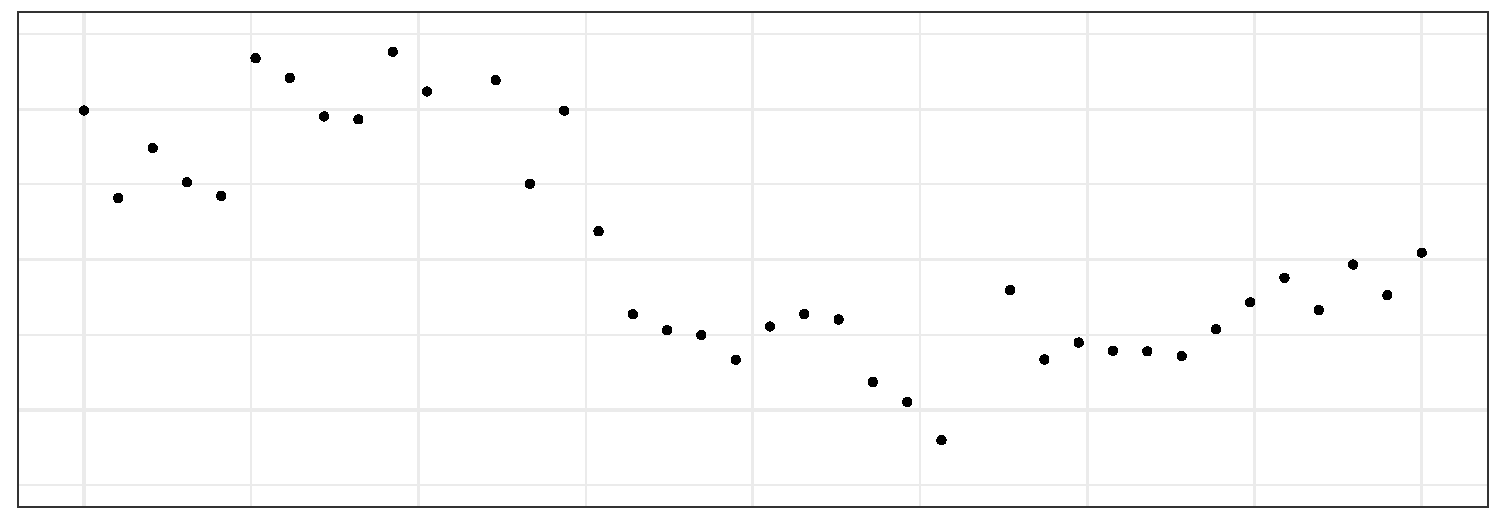
\includegraphics[height=1.4cm, width=6cm]{./plot/para1}     
    \end{figure}
    \item<+-> Fit null model $\hat{f}_1(\bx_1)$ using Kernel Ensemble
    \begin{figure}
	\centering
    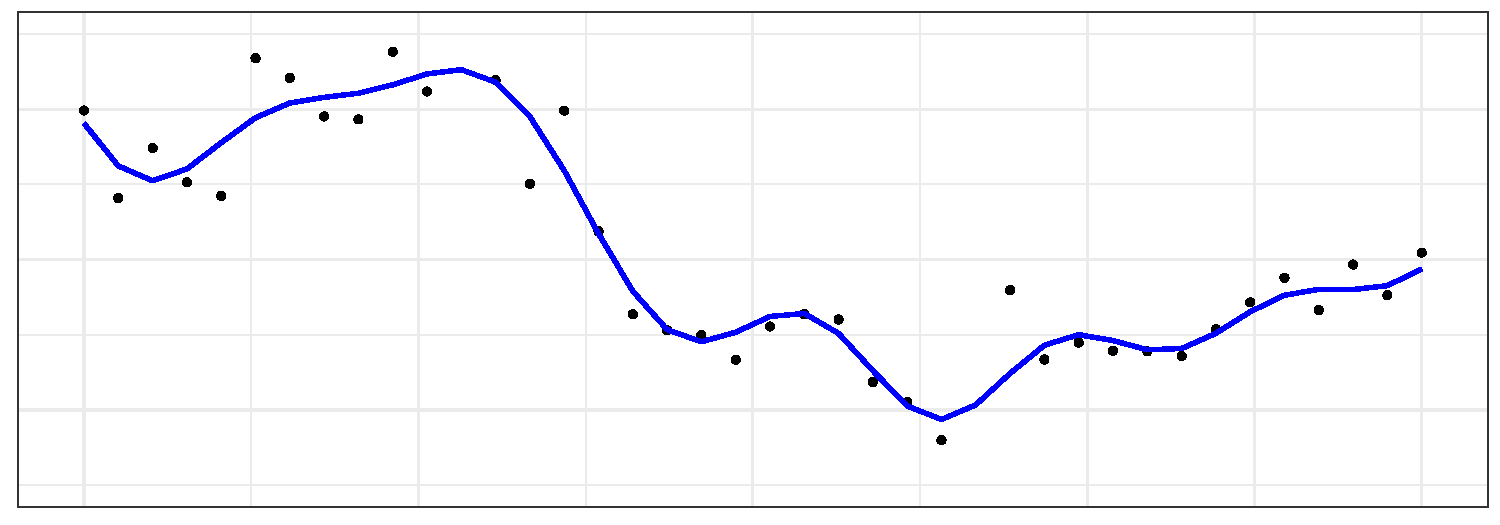
\includegraphics[height=1.4cm, width=6cm]{./plot/para2}     
    \end{figure}
    \item<+-> Generate many $y^*= \hat{f}_1(\bx_1) + \epsilon^*$, then generate $\hat{T}_0$'s based on $y^*$.
    \begin{figure}
	\centering
    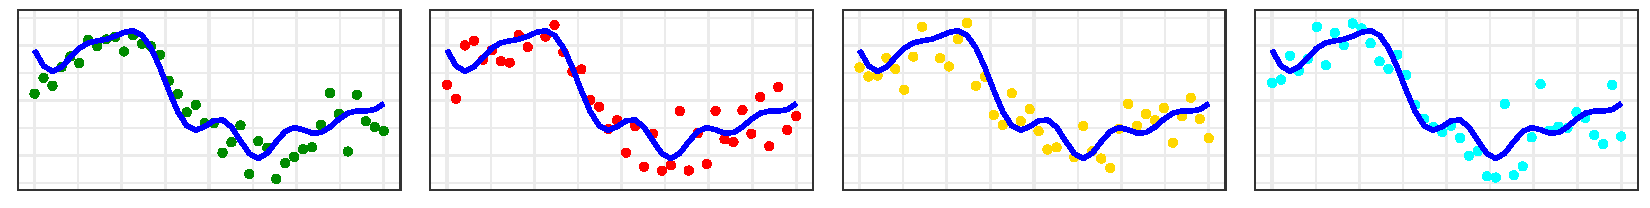
\includegraphics[height=1.4cm, width=10cm]{./plot/para_boot}         
    \end{figure}    
  \end{enumerate}
\end{frame}

\begin{frame}  
\frametitle{Bootstrap Test: Idea}
\begin{enumerate}
\item Notice the $\hat{T}_0$'s are generated under null
\item Therefore, bootstrap sample $\{\hat{T}_{0b}\}_{b=1}^B$ forms null distribution of $T$
\item Compute p-value is as simple as:
$$p\mbox{-value} = \frac{1}{B}\sum_{b=1}^B I(T_{obs} < \hat{T}_{0b})$$
\end{enumerate}
\begin{figure}
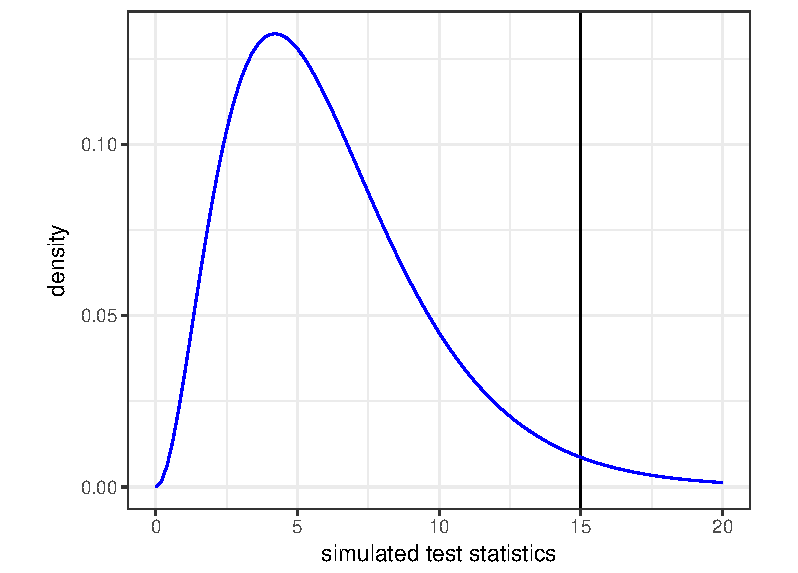
\includegraphics[width=0.68\textwidth, height=2.5cm]{./plot/p_value} 
\end{figure}
\end{frame}

\begin{frame}
\frametitle{Summary}
\begin{itemize}
\item \textbf{Data}: 
$\{ y_i, \bx_i \}_{i=1}^n, \quad \mbox{where} \quad 
\bx_i= \{\bx_{i1}, \bx_{i2}\}$
\item \textbf{Goal}: Test for $$\quad H_0: \quad f_2(\bx_{i2}) = 0$$
\item \textbf{Model}: {\color{red}\textbf{CVEK}}: Kernel Machine Regression + Ensemble Learning
$$\by =\bmu + \bK_1\balpha +\bepsilon$$
\item \textbf{Hypothesis Test}: {\color{red}\textbf{asym} or \textbf{boot}}: Variance Component Test
$$ T \propto \hat{\bepsilon}^\top \bK_2 \hat{\bepsilon}$$
\item Looks like we solved everything?
\begin{itemize}[<+->]
\item Robust null model fit using ensemble learning (CVEK).
\item Robust small sample test using bootstrap.
\item How does it perform though?
\end{itemize}
\end{itemize}
\end{frame}

\section{Simulation Study}
\begin{frame}  
\frametitle{Procedure}
\begin{enumerate}
\item generate data using a specific $k$: \[\by=\bmu + f_1(\bx_1)+\delta \cdot f_2(\bx_2) + \bepsilon.\]
\item fit $\by=\bmu + f_1(\bx_1) + \bepsilon$ with an ensemble of kernels $$\bk_{model}=\{k_1, k_2, k_3\}.$$
\item repeat steps 1 and 2 under
\begin{enumerate}
\item different data-generation mechanisms
\item different types of kernel ensembles $\bk_{model}$
\end{enumerate}
\end{enumerate}
\end{frame}

\begin{frame}  
\begin{itemize}
\item data I tried:
\begin{center}
 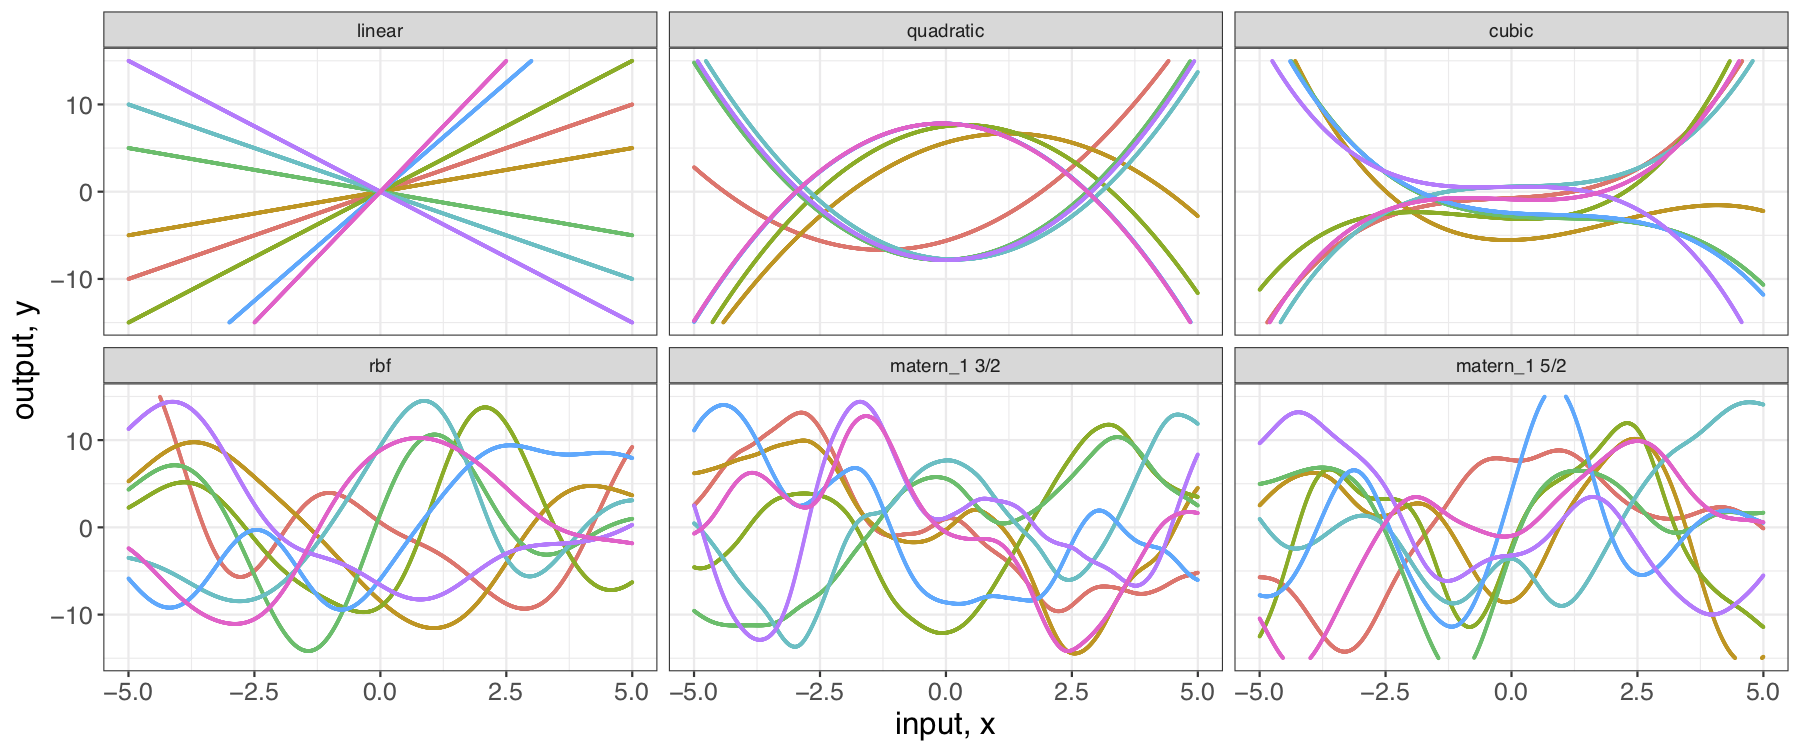
\includegraphics[height=3cm, width=10.6cm]{./plot/data_plot} 
\end{center}
\item first set of $\bk_{model}$ I tried (Polynomial Kernels):
\begin{center}
 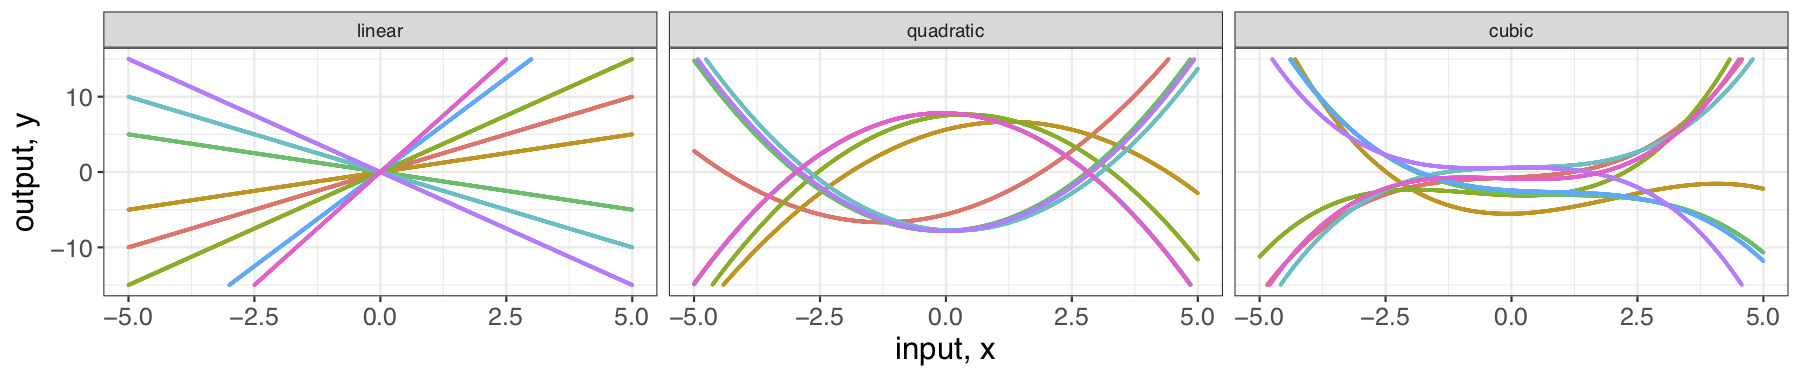
\includegraphics[height=1.5cm, width=10.6cm]{./plot/poly_lib} 
\end{center}
\end{itemize}
\end{frame}

\begin{frame}  
\begin{itemize}
\item data I tried:
\begin{center}
 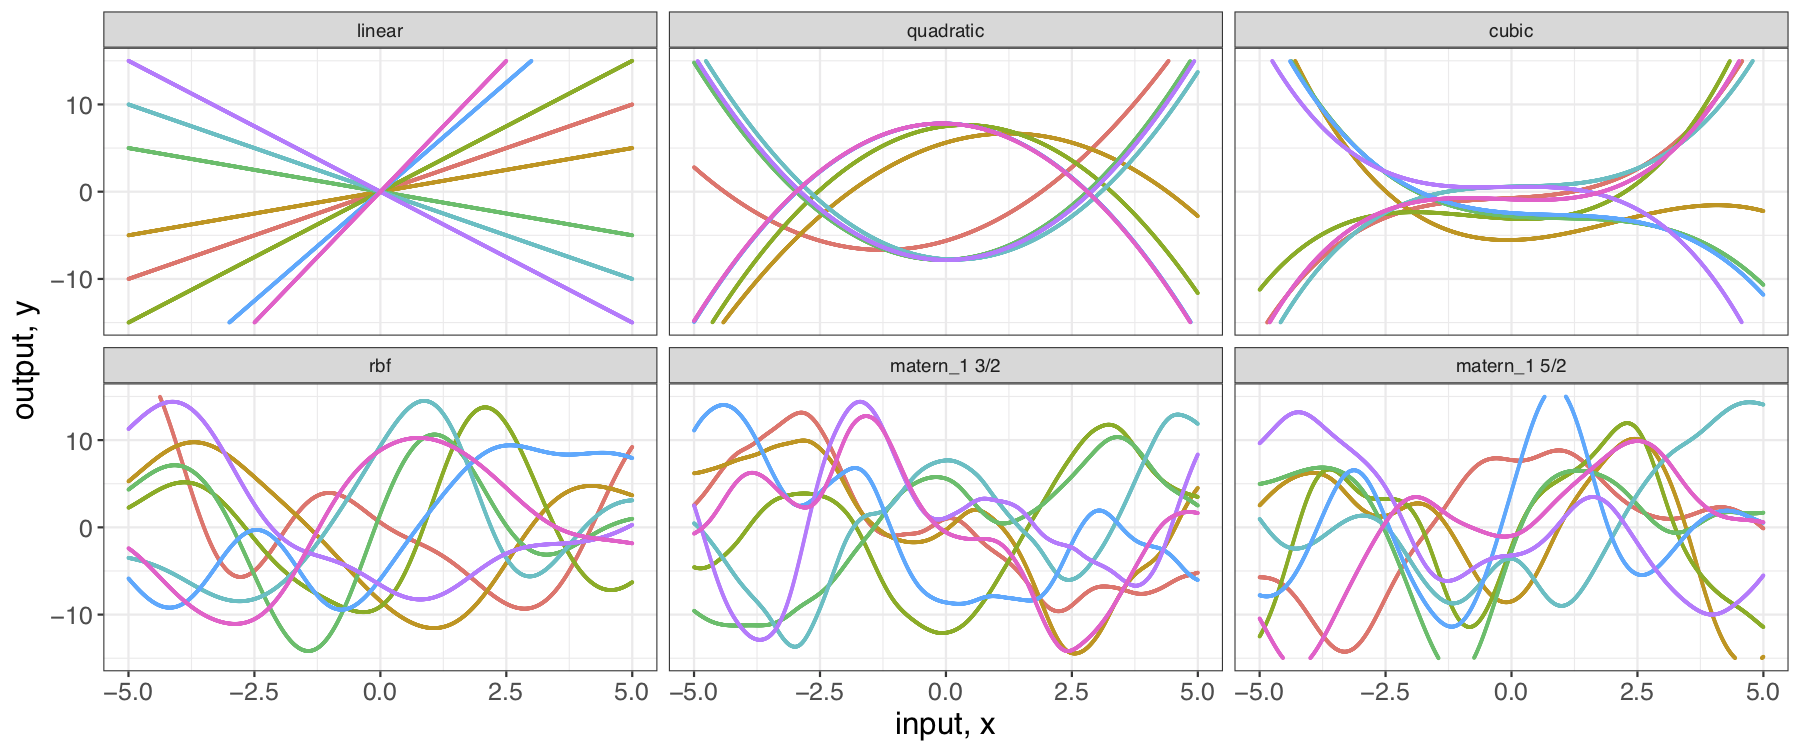
\includegraphics[height=3cm, width=10.6cm]{./plot/data_plot} 
\end{center}
\item second set of $\bk_{model}$ I tried (RBF Kernels):
\begin{center}
 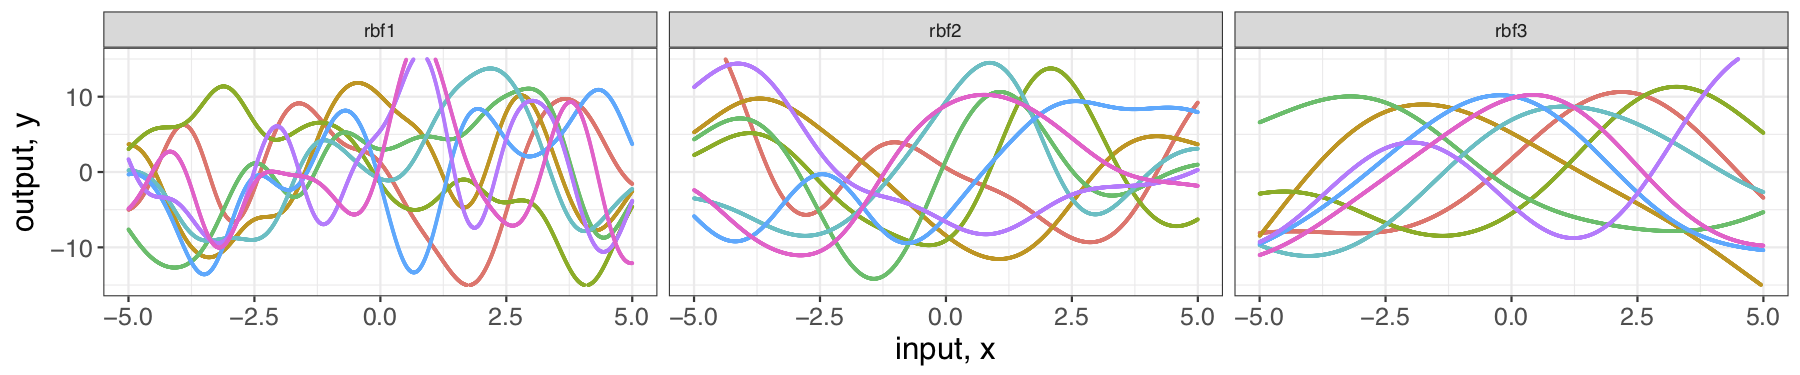
\includegraphics[height=1.5cm, width=10.6cm]{./plot/rbf_lib} 
\end{center}
\end{itemize}
\end{frame}

\begin{frame}  
\frametitle{Test Performance, Oracle Ensemble}
\begin{center}
 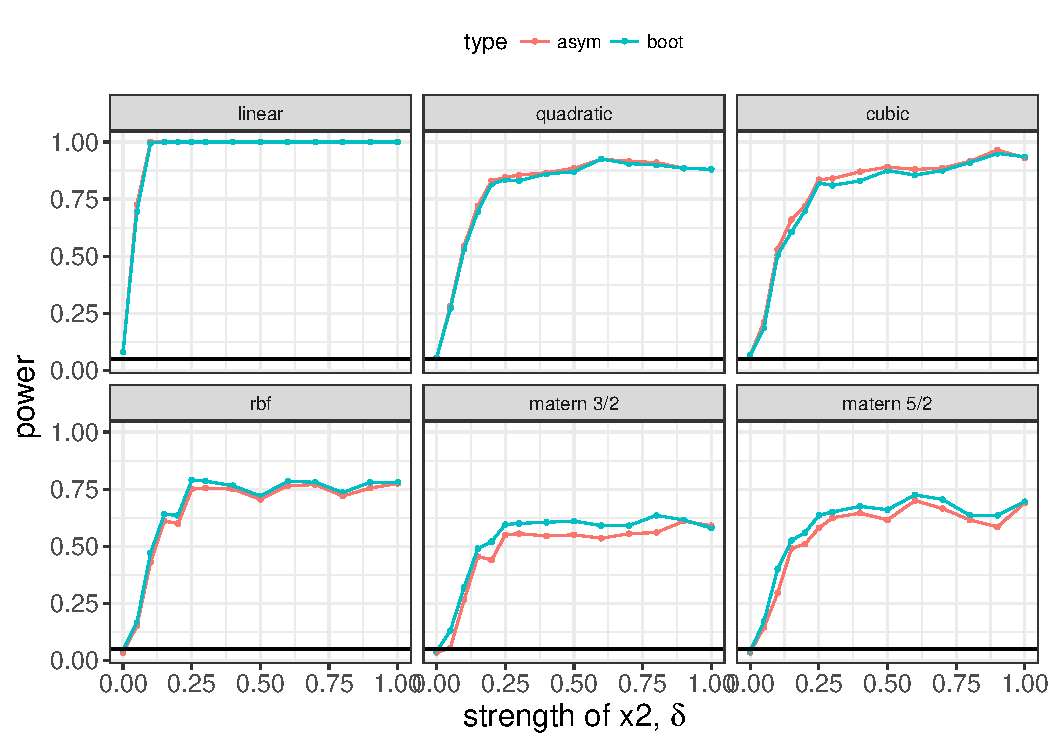
\includegraphics[height=6.4cm, width=10.6cm]{./plot/true_mod} 
\end{center}
\end{frame}

\begin{frame}  
\frametitle{Test Performance, Polynomial Ensemble}
\begin{center}
 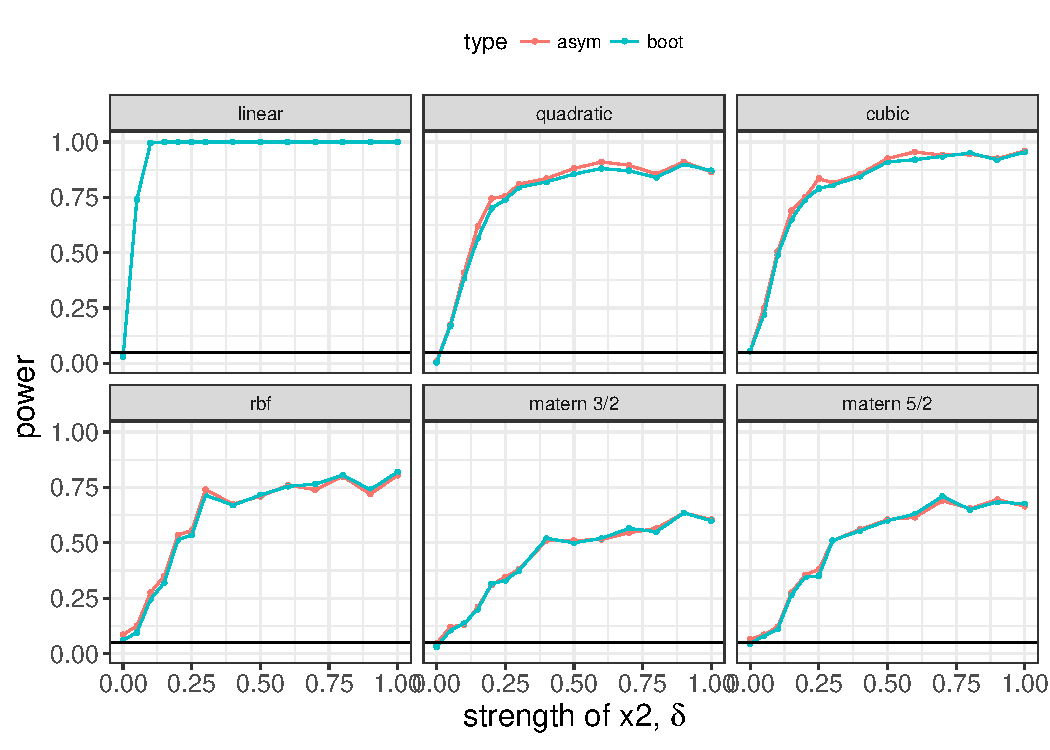
\includegraphics[height=6.4cm, width=10.6cm]{./plot/poly_mod} 
\end{center}
\end{frame}

\begin{frame}  
\frametitle{Test Performance, RBF Ensemble}
\begin{center}
 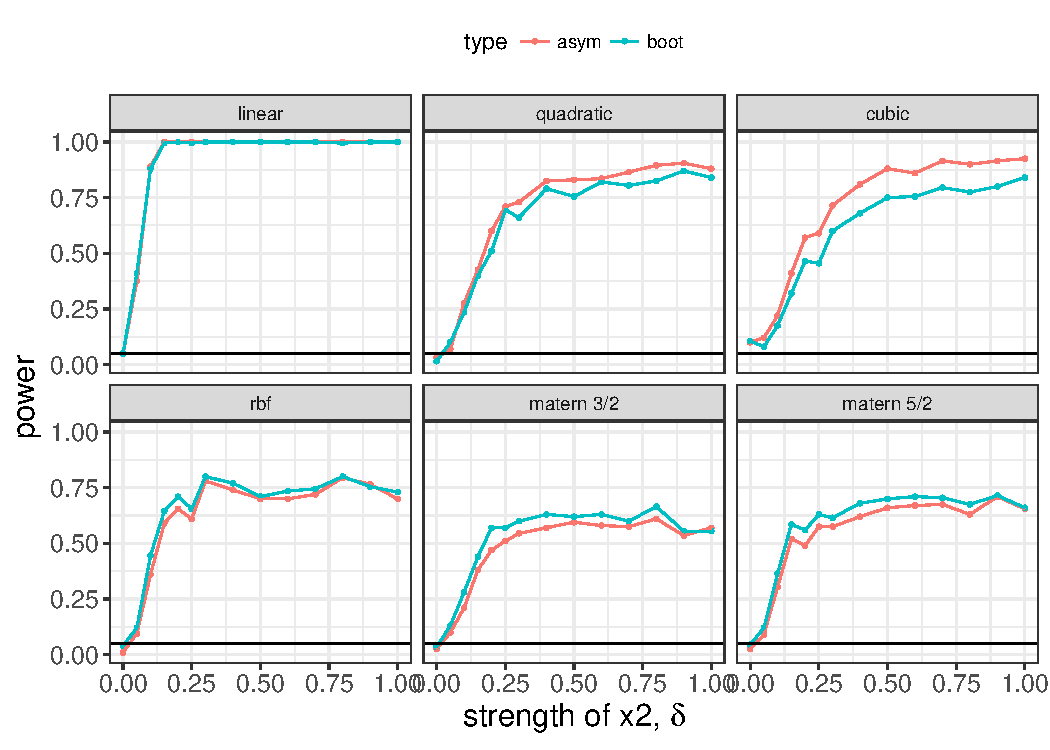
\includegraphics[height=6.4cm, width=10.6cm]{./plot/rbf_mod} 
\end{center}
\end{frame} 

\begin{frame}  
\frametitle{Conclusion}
\begin{enumerate}
\item better guarantee Type I error.
\item better power under non-polynomial (especially non-smooth) data.
\item R package \textit{CVEK} is coming soon! $\{https://github.com/IrisTeng/CVEK\}$
\end{enumerate}
\end{frame}

\begin{frame}  
\begin{center}
\textbf{Questions?}
\end{center}
\end{frame}

\section*{References \& Appendix}
\begin{frame}  
\frametitle{Main References}
\begin{enumerate}
\begin{small}
\item Lin X (1997). “Variance component testing in generalised linear models with random effects.”
\item Liu JZ, Coull B (2017). “Robust Hypothesis Test for Nonlinear Effect with Gaussian Processes.”
\item Maity A, Lin X (2011). “Powerful tests for detecting a gene effect in the presence of possible
gene-gene interactions using garrote kernel machines.”
\item Liu D, Lin X, Ghosh D (2007). “Semiparametric regression of multidimensional genetic
pathway data: least-squares kernel machines and linear mixed models.”
\item Hastie T, Tibshirani R, Friedman J (2009). The Elements of Statistical Learning: Data
Mining, Inference, and Prediction, Second Edition.
\item Press TM (2006). “Gaussian Processes for Machine Learning.”
\end{small}
\end{enumerate}
\end{frame}

\begin{frame}  
\frametitle{Appendix}
Linear $\Rightarrow$ Nonliear:
\begin{align*}
\hat{\by}&=\bX \hat{\bbeta}\\
&=\bX (\bX^\top \bX +\lambda I_p)^{-1}\bX^\top \by \tag{ridge regression}\\
&=\bX \bX^\top(\bX \bX^\top +\lambda I_n)^{-1}\by \tag{svd}\\
&=\bX \bX^\top \hat{\balpha}=\underset{n\times n}{\bK} \hat{\balpha}
\end{align*}
\end{frame}

\begin{frame}  
\begin{enumerate}
\item Obtain parameter estimates from the original data by fitting a null-hypothesis model \[\hat{\by}=\bK_0(\bK_0+\lambda \bI)^{-1}\by=\bA_0\by\]
\item Sample $\by^*$ for each individuals with a random noise, whose variance is also estimated.
\item Compute the test statistic, based on fitting the alternative-hypothesis model to the samples obtained in Step 2.
\item Repeat Steps 2 and 3 for $B$ times, to obtain an approximate distribution of the test statistic.
\item Compute the test statistic for the original data, based on fitting the alternative- hypothesis model.
\item Compute the $p$-value, by comparing the test statistic in Step 5 to the distribution in Step 4.
\end{enumerate}
\end{frame}

\end{document}